\section{Anterior introducción, borrar}
\todo{Borrar esta sección!}

% TODO -- borrar esto
Las \textbf{ideas principales} de este trabajo son dos. En primer lugar, resolver un problema de \textbf{reconocimiento facial invariante a cambios en la edad}, por sus siglas en inglés, \entrecomillado{AIFR}. Dentro de este problema, nos centraremos en resolver una tarea de \textbf{retrieval}. En segundo lugar, introducir una nueva técnica de aprendizaje automático, que busca \textbf{solucionar los principales problemas que plantea el uso de la función de pérdida \entrecomillado{triplet loss}} \cite{informatica:principal}. Esta técnica introduce una forma de generar los \textit{batches} de triples de forma \textit{online}. Esto evita tener un paso separado en el ciclo de entrenamiento, dedicado únicamente a volver a generar de forma \textit{offline} nuevos \textit{batches} de triples. Y de paso, se consigue normalizar la dificultad que suponen estos conjuntos de triples. Estudiaremos esta técnica detalladamente en \customref{isec:batching}.

Esta situación plantea una serie de \textbf{problemas}:

\begin{itemize}
    \item La nueva técnica que busca mejorar el uso de \textit{Triplet Loss} se plantea en un \textbf{ambiente completamente distinto} al de \textit{AIFR}, en concreto, en el ámbito de re-identificación de personas \cite{informatica:principal}
        \begin{itemize}
            \item En el problema de re-identificación de personas se trabaja normalmente con imágenes de cuerpo completo y con diferencias temporales entre imágenes muy acotadas. La tarea es seguir identificando con la misma identidad a una persona que ha desaparecido momentáneamente de la escena.
            \item Mientras que los problemas principales en \textit{AIFR} son otros (y se detallarán en \customref{ich:descrp_problema}). Buscamos asignar la misma identidad a imágenes faciales de una persona, tomadas en momentos muy distintos de su vida.
            \item Por tanto, no disponemos de literatura en la que se expongan resultados obtenidos de aplicar estas técnicas a nuestro ámbito de trabajo
        \end{itemize}
    \item Como veremos en \customref{ich:estado_arte}, no hay trabajos previos que hayan aplicado \textit{triplet loss} (y mucho menos la variación que introducimos) para resolver un problema de \textit{AIFR}. Por tanto, el acceso a literatura es todavía más restringido
    \item Esta técnica cambia fundamentalmente la forma de generar \textit{batches} de datos. Y por tanto, modifica en esencia muchas partes primarias del proceso de aprendizaje. Por ejemplo, el ciclo de entrenamiento, el cálculo de métricas durante el entrenamiento, el acceso a los datos... Es por este motivo que hemos tenido que realizar \textbf{implementaciones personalizadas de casi todos estos elementos}, sin poder hacer uso de la mayoría de implementaciones que ofrecen las librerías de aprendizaje automático. Esto supone que deberemos dedicar \textbf{mucho más tiempo del esperado a la implementación}, teniendo en cuenta que hay que prestar \textbf{especial atención a la optimización y validación} mediante \textit{tests} de estos nuevos módulos. Esto se plasma en \customref{ich:implementacion}
    \item Como comentaremos en \customref{ich:conclusiones}, este trabajo \textbf{no ha dado buenos resultados en la práctica}, comparado con otras técnicas más establecidas en el ámbito del \textit{AIFR}. Sin literatura que aplique nuestras nuevas técnicas en nuestro ámbito, como veremos en \customref{isec:interesareaestudio}, tenemos que \textbf{basarnos únicamente en todo el trabajo realizado para estudiar el por qué} de este mal comportamiento.
\end{itemize}

Aunque entraremos en detalle en \customref{isec:github_buenas_practicas}, todo el desarrollo del código y de la presente memoria se ha relaizado en un repositorio abierto de \textit{Github} \cite{informatica:repogithub}. Aquí se pueden consultar todos los \textit{commits}, \textit{pull requests}, \textit{issues}, \textit{feature branches} y la integración continua con \textit{Github Actions}.

La siguiente imagen ayuda a entender la diferencia entre el problema de re-identificación (ambiente en el que se introduce la mejora de \textit{triplet loss} que vamos a explorar) y el problema de \textit{AIFR}:

\begin{figure}[H]
    \centering
    \ajustarsubcaptions
    \begin{subfigure}{0.4\textwidth}
        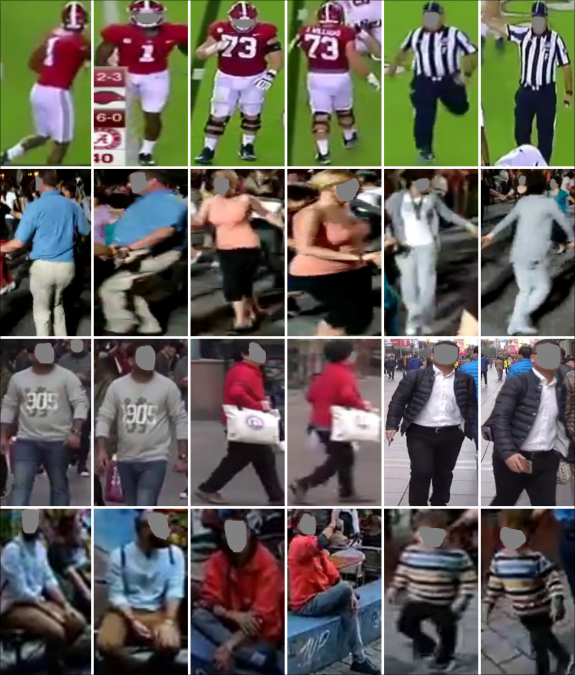
\includegraphics[width=0.9\textwidth]{informatica/ejemplo_reid}
        \caption{Ejemplo de un problema de re-identificación. Imágenes del \textit{dataset} \textit{LuPerson}. Imagen extraída de \cite{informatica:luperson}}
    \end{subfigure}%
    \begin{subfigure}{0.6\textwidth}
        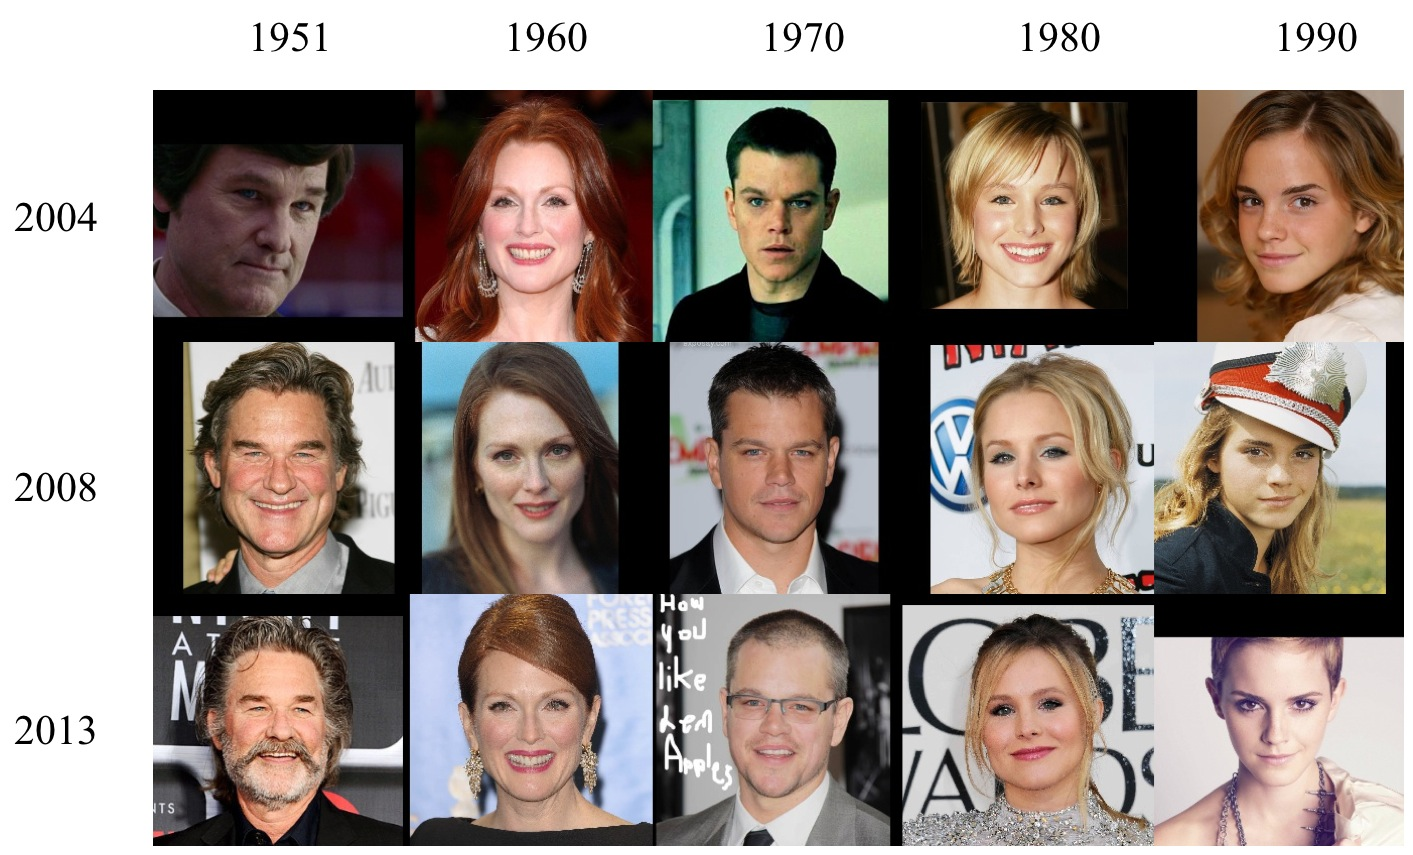
\includegraphics[width=0.9\textwidth]{informatica/cacd_example}
        \caption{Ejemplo de un problema de \textit{AIFR}. Imágenes del \textit{dataset} \textit{CACD}. Imagen extraída de \cite{informatica:paper_cacd}}
    \end{subfigure}

    \caption{En el ejemplo de re-identificación podemos observar pares de imágenes, de cuerpo completo, de una persona en dos instantes de tiempo muy cercanos (misma ropa, prácticamente el mismo fondo). Además, en ese ejemplo el \textit{dataset} borra información sobre el rostro de las personas. En el ejemplo de \textit{AIFR}, podemos ver varias imágenes de una persona en distintos momentos de su vida, con años de diferencia. Nos centramos en la información de la cara de las personas. La variabilidad se centra en cambios en los rasgos faciales por el paso de los años, no se usa la misma ropa, ...}
\end{figure}

